\documentclass[11pt]{article}

\usepackage[preprint]{acl}

\usepackage{times}
\usepackage{latexsym}

\usepackage[T1]{fontenc}
\usepackage[utf8]{inputenc}

\usepackage{microtype}
\usepackage{inconsolata}
\usepackage{graphicx}
\usepackage{amsmath}
\usepackage{amssymb}
\usepackage{booktabs}
\usepackage{enumitem}
\usepackage{tikz}
\usetikzlibrary{positioning,arrows.meta}

\newcommand{\mask}{\ensuremath{\mathrm{m}}}
\newcommand{\keep}{\textsc{keep}}
\newcommand{\edit}{\textsc{edit}}
\newcommand{\drop}{\textsc{drop}}
\newcommand{\maskdisc}{\textsc{[mask]-disc}}

\title{DiffusEdit: Final Proposal}

\author{
  \textbf{Tatva Agarwal\textsuperscript{*}} \\ 2024117005 \And
  \textbf{Vedant Kulkarni\textsuperscript{*}} \\ 2024101140 \And
  \textbf{Bysani Vedavyas\textsuperscript{*}} \\ 2024101025 \And
  \textbf{Venya Velmurugan\textsuperscript{*}} \\ 2024114002
}

\begin{document}

\maketitle

\renewcommand{\thefootnote}{\fnsymbol{footnote}}
\footnotetext[1]{Equal contribution; authors listed alphabetically.}
\renewcommand{\thefootnote}{\arabic{footnote}}
\setcounter{footnote}{0}

\begin{abstract}
Reference articles go out of date as events develop, and updating them by hand is slow. Regenerating the article with a language model automates the update, but rewrites text that was already correct and leaves no record of what changed. DiffusEdit instead edits the article in place. Small trained layers, reading the hidden states of a frozen masked diffusion language model, decide which sentences to keep, edit, or delete, and which tokens inside them are stale. The frozen model rewrites only the stale positions, and the system repeats the process on sentences that the rewrites themselves made wrong. Training labels come from pairs of Wikipedia snapshots, and evaluation measures update quality, faithfulness, minimality, and coverage of the cascading edits.
\end{abstract}

\section{Introduction}
\label{sec:intro}

Reference text goes out of date. A Wikipedia article about a factory fire may say that three people died and that the small death toll limited the political fallout. A week later, news reports revise the toll to forty-two. The first sentence is contradicted directly, but the second is wrong since it rests on a fact that no longer holds. We call the second kind of required change a \emph{cascading edit}, a sentence that must change only because another sentence changed.

DiffusEdit updates the article in place. Small trained heads over a frozen masked diffusion model choose the stale sentences and tokens, the model infills only those positions, and the loop repeats on sentences the repairs themselves broke. On the fire example, round one masks \emph{three} and infills \emph{forty-two}, and round two rewrites the fallout sentence the first repair left unsupported.

\section{Task Definition}
\label{sec:problem}

An article is a sequence of sentences $A = (s_1, \dots, s_n)$, new evidence arrives as a set of text snippets $E = (e_1, \dots, e_m)$, and the system must produce an updated article $\hat{A}$ from the two alone. Faithfulness requires every claim in $\hat{A}$ to agree with the evidence and the untouched parts of the article, coverage requires every evidence fact that bears on the article to appear in $\hat{A}$, and minimality requires $\hat{A}$ to stay close to $A$. None of the three is computable, so the metrics of Section~\ref{sec:eval} stand in for them. We say $s_j \rightsquigarrow s_k$ when changing $s_j$ forces a change in $s_k$ even though the evidence says nothing about $s_k$ directly.

\section{Related Work}
\label{sec:related}

Early evidence-driven correction handles one sentence or claim at a time, masks the tokens that a new fact contradicts and refills them \citep{shah-etal-2020-automatic, thorne-vlachos-2021-evidence}. Closest to us, FRUIT \citep{iv-etal-2022-fruit} defines the task this project works on, and its EDIT5 model writes the updated article left to right while copying unchanged sentences through special tokens.

EditPropBench \citep{kruthof-2026-editpropbench} measures how many required downstream changes a model finds after a planted edit, and the strongest prompted model tested misses about 30\% of them when the dependence is implicit. HiCaM \citep{shi-etal-2025-hicam} propagates a change by having a prompted model build an entity graph and a summary tree of the document.

In diffusion decoding, several works reconsider tokens the sampler already committed \citep{wang-etal-2025-remasking, bie-etal-2026-llada21}. \citet{yao-2026-remask} argue for re-masking such tokens instead of overwriting them, and we reuse their per-position re-masking cap. Detect, Remask, Repair \citep[DRR;][]{zou-etal-2026-detect} is a prior system that applies a diffusion model to existing text and external evidence. It scores each token of a stale summary with \maskdisc{}, a linear classification head over the diffusion model's hidden states, then masks and infills the highest-scoring tokens, re-scoring the summary over several rounds. Our work extends this system.

\section{Motivation}
\label{sec:motivation}

The shortcomings of existing work are as follows.

\emph{Cascades are not modeled.} DRR detects tokens that clash with the evidence, on summaries of about ninety tokens. A cascading edit clashes only with another sentence that changed, so scoring against the evidence has no signal for it, and nothing in the design tracks which sentences depend on which.

\emph{Infilling cannot delete.} Every mask must be filled by exactly one token, so a system built on infilling alone can rewrite a sentence but never remove it.

\emph{No token-level supervision exists.} FRUIT-WIKI pairs outdated and updated articles without labeling which tokens went stale, and DRR trains on short synthetic summaries, so article-scale training data must be derived.

\section{Contributions}
\label{sec:contributions}

The contributions address these shortcomings.

\begin{enumerate}[label=(\alph*)]
\item A sentence-level \keep{}/\edit{}/\drop{} classifier over pooled hidden states, which restricts token scoring to \edit{} sentences and adds deletion through \drop{}.
\item An iterative edit loop that returns broken sentences to the pipeline, comparing three cascade detectors: mention overlap, staleness delta, and a learned consequence head.
\item Variable-length repair through multi-length infilling and reranking for fluency and evidence support.
\item Sentence- and token-level staleness labels derived from FRUIT-WIKI by alignment, plus a mined and hand-checked set of cascade pairs.
\item An evaluation separating detection quality, update quality, minimality, and cascade recall, with baselines, oracles, and ablations.
\end{enumerate}

\section{Proposed Methodology}
\label{sec:method}

DiffusEdit builds on a frozen masked diffusion language model, LLaDA-8B \citep{nie-etal-2025-llada}, with Dream \citep{ye-etal-2025-dream} as a drop-in alternative. Such a model predicts the original token at every masked position, using the visible tokens on both sides, so it can infill exactly the positions we mask. One forward pass over the evidence and the article yields a hidden state $h_i \in \mathbb{R}^d$ per token, and everything DiffusEdit trains is a small head reading these vectors. Figure~\ref{fig:pipeline} shows one round. The loop ends when nothing is flagged or budgets stop it.\footnote{Every numeric value in this proposal is a starting point for validation rather than a final choice.}

\begin{figure}[t]
\centering
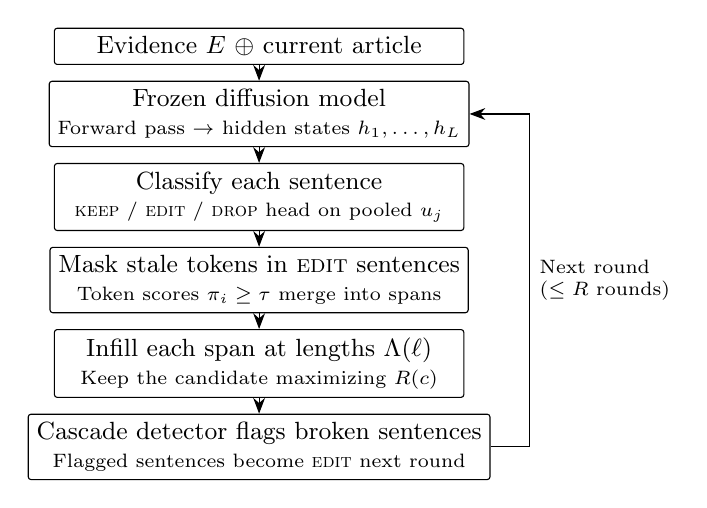
\begin{tikzpicture}[
  node distance=2mm,
  box/.style={draw, rounded corners=1pt, align=center, font=\small, inner sep=3pt, minimum width=5.2cm},
  >={Stealth[length=2mm]}
]
\node[box] (input) {Evidence $E$ $\oplus$ current article};
\node[box, below=of input] (model) {Frozen diffusion model\\[-1pt] {\scriptsize Forward pass $\rightarrow$ hidden states $h_1, \dots, h_L$}};
\node[box, below=of model] (cls) {Classify each sentence\\[-1pt] {\scriptsize \keep{} / \edit{} / \drop{} head on pooled $u_j$}};
\node[box, below=of cls] (mask) {Mask stale tokens in \edit{} sentences\\[-1pt] {\scriptsize Token scores $\pi_i \ge \tau$ merge into spans}};
\node[box, below=of mask] (infill) {Infill each span at lengths $\Lambda(\ell)$\\[-1pt] {\scriptsize Keep the candidate maximizing $R(c)$}};
\node[box, below=of infill] (casc) {Cascade detector flags broken sentences\\[-1pt] {\scriptsize Flagged sentences become \edit{} next round}};
\draw[->] (input) -- (model);
\draw[->] (model) -- (cls);
\draw[->] (cls) -- (mask);
\draw[->] (mask) -- (infill);
\draw[->] (infill) -- (casc);
\draw[->] (casc.east) -- ++(5mm,0) |- (model.east)
  node[pos=0.25, right, font=\scriptsize, align=left] {Next round\\($\le R$ rounds)};
\end{tikzpicture}

\caption{One round of DiffusEdit.}
\label{fig:pipeline}
\end{figure}

\subsection{Scoring Heads}
\label{sec:heads}

For sentence $s_j$ covering positions $\mathcal{I}_j$, heads that judge whole sentences read the mean-pooled vector
\begin{equation}
u_j \;=\; \frac{1}{|\mathcal{I}_j|} \sum_{i \in \mathcal{I}_j} h_i
\label{eq:pool}
\end{equation}
The alternatives are max pooling, which keeps each dimension's largest value, and attention pooling, where a learned query weights each token.

\paragraph{Sentence classifier.}
A linear layer maps $u_j$ to three probabilities,
\begin{equation}
p_j \;=\; \mathrm{softmax}\!\left(W_c\, u_j + b_c\right)
\label{eq:cls}
\end{equation}
A wrong deletion is permanent, so a sentence is deleted only when its \drop{} probability clears a confidence gate $\tau_d$, and otherwise it is treated as \edit{}. Since most sentences are \keep{}, the loss is weighted by inverse class frequency.

\paragraph{Token staleness scoring.}
The token scorer, following \maskdisc{}, is a linear layer with a sigmoid output on each token's hidden state,
\begin{equation}
\pi_i \;=\; \sigma\!\left(w_d^\top h_i + b_d\right)
\label{eq:token}
\end{equation}
read as the probability that token $i$ is stale. Derived labels come from diffing aligned sentence pairs token by token (Section~\ref{sec:data}). Synthetic corruptions follow \citet{zou-etal-2026-detect}: we mask 30--70\% of a correct article's tokens, let the frozen model refill them conditioned on the \emph{outdated} evidence, and label a refilled token stale when it differs from the original.

\paragraph{Consequence prediction.}
The third head predicts a yes or no value, for an ordered pair of sentences, that decides whether the second must change given that the first just changed. It applies an MLP with one hidden layer of width 512 to the pooled vectors of the two sentences, scoring the pair as
\begin{equation}
g_{jk} \;=\; \sigma\!\Big(\mathrm{MLP}_\psi\big([\,u_j;\; u_k;\; u_j \odot u_k;\; |u_j - u_k|\,]\big)\Big)
\label{eq:cons}
\end{equation}

\subsection{Edit Loop}
\label{sec:inference}

\paragraph{Variable-length infilling.}
Each round opens with a fresh forward pass over the current text, and inside each \edit{} sentence the tokens with $\pi_i \ge \tau$, capped at half the sentence, merge into contiguous spans. A span of $\ell$ masks yields exactly $\ell$ tokens, and the correct replacement is often shorter or longer, so each span is infilled at every length in
\begin{equation}
\Lambda(\ell) \;=\; \{\,0,\; \lceil \ell/2 \rceil,\; \ell,\; \ell + 2,\; 2\ell\,\}
\label{eq:lambda}
\end{equation} Length zero deletes the span without deleting its sentence, and it wins only when it beats the best rewrite by a tuned margin, since deletion also removes the claim from the verifier's check. Candidates are scored for fluency by the masked pseudo-log-likelihood $\mathrm{PLL}$, the average log-probability the frozen model assigns to each token when that token alone is masked, and for support by a fact verifier trained on VitaminC \citep{schuster-etal-2021-vitaminc}, taking the maximum over evidence snippets. The two combine into
\begin{equation}
R(c) \;=\; \lambda\, \mathrm{PLL}(s^{c}) + (1 - \lambda)\, \mathrm{Ent}(s^{c}, E)
\label{eq:rerank}
\end{equation}
where $s^c$ is the sentence after substituting candidate $c$ and $\lambda$ comes from a validation grid. If reranking proves weak, the fallback is reward steering, which guides the sampler toward supported text.

\paragraph{Cascade detectors.}
We will compare three detectors.

\begin{enumerate}[label=(\alph*)]
    \item Mention overlap defines a mention extractor $M$ that returns the named entities, numbers, and dates of a text (via spaCy). This flags $s_k$ when $M(s_k)$ shares a string with the mentions of the sentences repaired this round.
    \item Staleness delta re-scores every token under the recomputed hidden states and flags $s_k$ when one of its tokens newly enters the top tenth of the article's token scores with $\pi_i \ge \tau_2$.
    \item Consequence prediction flags $s_k$ when the consequence score $g_{jk}$ passes a threshold $\tau_c$ for any repaired $s_j$. Only this detector can catch dependence without shared surface mentions.
\end{enumerate}

The round count is capped at $R = 3$, and each position may be re-masked at most $C_{\max} = 3$ times.

\section{Dataset}
\label{sec:data}

\paragraph{FRUIT-WIKI.}
FRUIT-WIKI \citep{iv-etal-2022-fruit} is built by diffing the introductory sections of English Wikipedia between yearly snapshots and attaching evidence snippets from elsewhere in the encyclopedia. Its labels are distantly supervised, meaning an automatic procedure inferred them and no human checked them. Such labels are called \emph{silver} and human-verified labels \emph{gold}, and we train and tune on silver and report on gold only. The FRUIT authors estimate that only about a third of silver edits are supported by their attached evidence. We will first try to rebuild the dataset from 2026 snapshots taken six months apart, which would also postdate the frozen model's training data, and if that fails we will fall back to the original release.

\paragraph{Filtering.}
We filter to instances whose tokenized evidence and article fit in 1024 tokens and whose update modifies or removes at least one existing sentence, because inserting a sentence needs a placement decision our design does not make. Held-out silver articles form the validation set for threshold tuning.

\paragraph{Label derivation.}
Source and target sentences are aligned greedily by the F1 overlap of their token multisets. A source sentence with similarity at least $0.95$ is \keep{}, a match with at least $0.35$ is \edit{}, and an unmatched source sentence is \drop{}. Inside every \edit{} pair, a token-level diff marks the tokens the revision replaced or removed as stale. Alignment will mistake some heavy rewrites for a deletion plus an addition, so we will audit one hundred aligned articles by hand before training. If that failure is frequent, we will switch to a character-level F-score and re-derive the labels.

\paragraph{Cascade pair mining.}
An edited sentence is direct when the mentions it changed share a string with the evidence's mentions, and every other changed sentence is either a cascade or a stylistic rewrite. We hand-label several hundred from the gold articles as the cascade evaluation set, split by whether they share a mention with a direct edit, with consequence prediction measured on the group that does not. Training pairs are mined separately, by meaning rather than shared mentions, since a cascade often paraphrases the changed fact. Each edited sentence is represented by the tokens its revision changed, and a changed-but-not-direct sentence pairs with a direct edit of the same article when their changed tokens are close under a sentence encoder. We will check two hundred mined pairs by hand before training. If fewer than about sixty percent are real cascades, we drop the consequence head.

\section{Evaluation Plan}
\label{sec:eval}

\paragraph{Update quality.}
Let $U(\cdot)$ select an article's updated sentences, those with no exact match in $A$. UpdateROUGE \citep{iv-etal-2022-fruit}, the primary quality metric, computes ROUGE-1, -2, and -L between $U(\hat{A})$ and $U(A^\ast)$. Entity precision and recall compare $M(U(\hat{A}))$ with $M(U(A^\ast))$, and we count the unsupported entity tokens, those appearing in neither the original article nor the evidence. Faithfulness is AlignScore \citep{zha-etal-2023-alignscore} between $U(\hat{A})$ and the evidence.

\paragraph{Minimality, detection, and cascades.}
Minimality is the normalized token edit distance between $\hat{A}$ and $A$, plus the fraction of gold-\keep{} sentences reproduced verbatim. Detection quality is macro-F1 of the sentence classifier and area under the precision-recall curve of the token scorer. Cascade recall is the fraction of hand-labeled cascade sentences the active detector flags in any round. These metrics penalize a correct update phrased differently from the gold reference, so we will also read fifty outputs and tally errors.

\paragraph{Baselines, oracles, and ablations.}
Copy returns $A$ unchanged and anchors minimality. Full regeneration has the frozen sampler write a complete updated article into an all-\mask{} block, the same model with no editing. The fine-tuned editor is a T5 model trained on our silver split in the style of EDIT5, the published approach on this data. The prompted model, an instruction-tuned autoregressive model of comparable size, shows what prompting alone achieves. The no-evidence control runs the full pipeline with the evidence deleted, so whatever it still fixes comes from the model's memory. Four oracle runs each replace one stage's predictions with the true answers, showing what that stage's errors cost. Table~\ref{tab:ablations} lists the ablation grid, each row varying one axis on 200 gold articles.

\begin{table}[t]
\caption{Ablation axes. Defaults in bold.}
\label{tab:ablations}
\centering
\small
\begin{tabular}{ll}
\toprule
Axis & Values \\
\midrule
Cascade detector & none, (a), \textbf{(b)}, (c) \\
Rounds $R$ & 1, 2, \textbf{3}, 4 \\
Candidate lengths $\Lambda$ & $\{\ell\}$, $\{0, \ell\}$, \textbf{full} \\
Detector training data & synthetic, derived, \textbf{mix} \\
Reranker & PLL, verifier, \textbf{combined} \\
Deletion margin & off, \textbf{on} \\
Cascade mining & string overlap, \textbf{embedding} \\
\bottomrule
\end{tabular}
\end{table}

\paragraph{Success criteria and validity.}
With a cascade detector on, cascade recall and UpdateROUGE on cascade sentences must exceed the single-round numbers. DiffusEdit must beat its no-evidence control, since the model has likely seen the Wikipedia articles. Every comparison carries a significance test over per-article scores.

\section{Risks and Limitations}
\label{sec:risks}

The main risk is that evidence may not steer the frozen generator, since it was never trained to let a snippet override nearby fluent text. DRR reports repair only on short summaries, and article length is untested.

The synthetic stream could teach the scorer to recognize model-generated text rather than evidence contradiction. Consequence prediction could read the changed sentence before or after its rewrite, and we start with after, which the dependent sentence must now agree with. And a cascade whose fix is a new sentence cannot be repaired without a placement head.

\bibliography{citations}

\end{document}
